\documentclass[18pts]{article}
\usepackage{amssymb,amsmath,latexsym,enumerate,graphicx,fullpage,url,multicol,longtable,color}
\usepackage{graphicx, tikz}
\usetikzlibrary{calc,shadows}
\usepackage[T1]{fontenc}
\usepackage{eso-pic,fancybox}
\usepackage[absolute,overlay]{textpos}
\usepackage{color}
\usepackage{mathptmx}
\usepackage{fix-cm}

%    \topmargin 0 in
%    \textheight 11in
%    \textwidth 6.25 in
%    \oddsidemargin 1in   % read Lamport p.163
%    \evensidemargin 1 in
%    \headsep = 20pt
\usepackage{anyfontsize}
\usepackage{xparse}

% suppresses hyphenation and aligns left
\usepackage[none]{hyphenat}
\raggedright


\newcommand\ProjectName[1]{
{
\fontsize{35}{40}\selectfont
\noindent\textbf{#1}\par
}
\vskip 2mm
\fontsize{20}{25}\selectfont
}

\newenvironment{justified}
{
\tolerance=1
\emergencystretch=\maxdimen
\hyphenpenalty=10000
\hbadness=10000
}


\renewcommand\large{
\noindent\fontsize{16}{19}\selectfont}
\renewcommand\Large{
\noindent\fontsize{18}{20}\selectfont}


%%%%%%%%%%%%%%%%%%%%%%%%%%%%%%%%%%%%%%%%%%%%%%%%%%%%%%
%
%					DO NOT CHANGE ANY ABOVE FORMAT/MACRO
%
%%%%%%%%%%%%%%%%%%%%%%%%%%%%%%%%%%%%%%%%%%%%%%%%%%%%%%
\begin{document}

\ProjectName{Hyperbolic Space on the Oculus Rift}
\noindent\textbf{Faculty Mentor: {
Pierre Albin} 
}
\vskip 2mm
\noindent\textbf{Team Leader:
{Daan Michiels}
}
\vskip 2mm
\noindent\textbf{Scholars: 
{Kyle McDaniel, Daniel Pugliese, Byron Wooden}
}\\

% There should really be some vertical space here!
% \vspace{0.5em}

\Large

\begin{justified}

Since the discovery of non-euclidean geometry in the early 19th century many mathematicians have explored hyperbolic space using pen and paper.
The goal of this project is to visualize 3-dimensional hyperbolic space as it would look to an inhabitant, using computer software. We use techniques from modern computer games and adapt them to hyperbolic geometry to walk around in this curved space.
Apart from a regular computer screen, the software can use the \emph{Oculus Rift}, a virtual reality device to show an immersive 3-dimensional image.

\begin{center}
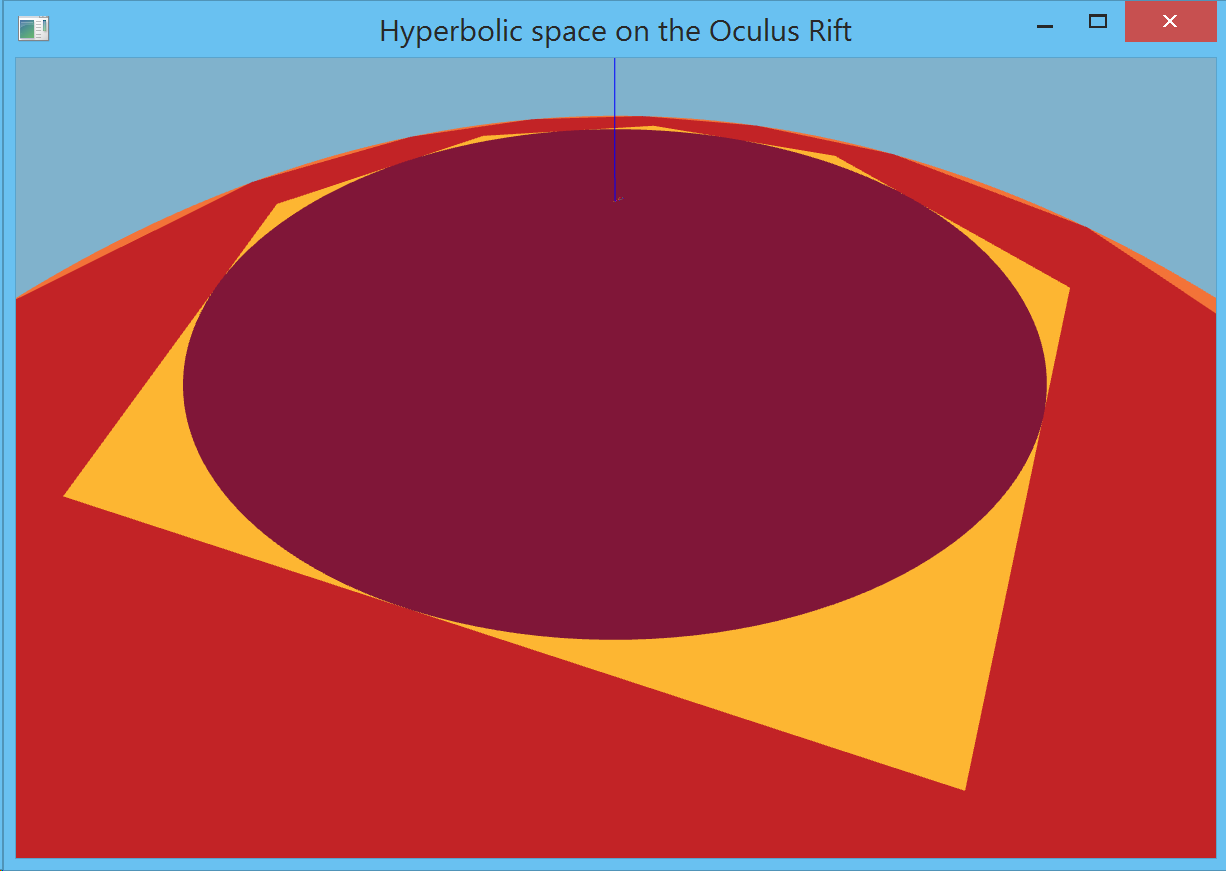
\includegraphics[width=0.49\linewidth]{ngons.png}
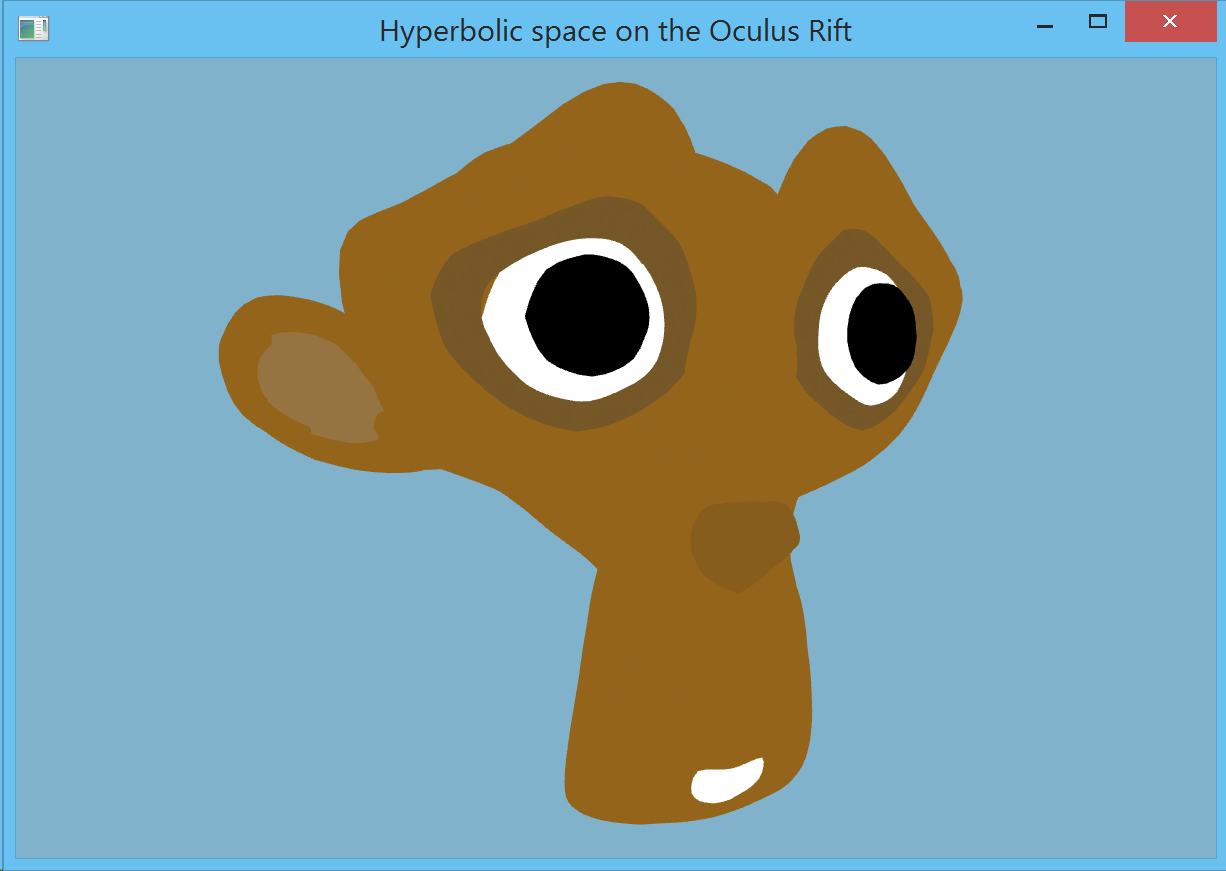
\includegraphics[width=0.49\linewidth]{suzy.png}
\end{center}

% In this second semester of the project, we have vastly improved the graphics and incorporated limited interaction with the world.
% Many interesting phenomena can be observed due to the curvature: the angles of a triangle do not sum to $180^\circ$, composing two translations does not always give a translation, objects get smaller exponentially with distance (instead of linearly).
 
\end{justified}

\end{document}
